\documentclass[12pt,a4paper]{article}
\usepackage[utf8]{inputenc}
\usepackage[russian]{babel}
\usepackage{amsmath, amssymb, amsfonts}
\usepackage{graphicx}
\usepackage{float}
\usepackage{geometry}
\geometry{left=2.5cm, right=2cm, top=2cm, bottom=2cm}
\usepackage{indentfirst}
\usepackage{caption}
\usepackage{subcaption}

\begin{document}

\title{\begin{center}Лабораторная работа № 5.1.3\end{center}
Эффект Рамзауэра}
\author{Струков О. И. \\ Б04-404}
\date{}

\thispagestyle{empty}
\pagenumbering{gobble}
\maketitle
\newpage
\pagenumbering{arabic}


\section*{Теоретическая часть}

\subsection*{1. Эффект Рамзауэра}
Эффект Рамзауэра --- аномальное поведение сечения упругого рассеяния медленных электронов на атомах инертных газов. В классической физике сечение рассеяния должно монотонно убывать с ростом энергии электрона (обратно пропорционально скорости). Однако экспериментально обнаружено, что при определённых энергиях (порядка нескольких эВ) сечение рассеяния резко падает, достигая минимума, а затем снова возрастает.

Это явление получило объяснение в квантовой механике. Электрон рассматривается как волна де Бройля, которая испытывает дифракцию на атоме. Атом моделируется как потенциальная яма глубиной $U_0$ и радиусом $l$. При определённых энергиях электронов возникает резонансное прохождение через потенциальную яму, аналогичное просветлению оптики в тонких плёнках.

\subsection*{2. Модель потенциальной ямы}
В простейшей модели атом представляется как сферическая потенциальная яма:
\begin{equation}
    U(r) = \begin{cases}
        -U_0, & r < l \\
        0, & r > l
    \end{cases}
\end{equation}
где $U_0$ --- глубина ямы, $l$ --- её радиус (размер электронной оболочки атома).

Решая уравнение Шрёдингера для этой задачи, можно найти коэффициент прохождения электрона через яму. Максимумы коэффициента прохождения (минимумы сечения рассеяния) возникают при условии:
\begin{equation}
    k_2 l = n\pi, \quad n = 1, 2, 3, \ldots
\end{equation}
где $k_2 = \sqrt{2m(E + U_0)}/\hbar$ --- волновое число внутри ямы, $E$ --- кинетическая энергия электрона вне ямы.

Отсюда энергия электронов, соответствующая $n$-му максимуму прохождения:
\begin{equation}
    E_n = \frac{\hbar^2 \pi^2 n^2}{2ml^2} - U_0.
\end{equation}

% % === МЕСТО ДЛЯ ВСТАВКИ СХЕМЫ ===
% \begin{figure}[htbp]
%     \centering
%     % \includegraphics[width=0.7\textwidth]{ramzauer_potential.png}
%     \fbox{\parbox{0.7\textwidth}{\centering\vspace{2cm} \textit{Вставьте сюда Рис. 1 из методички: Модель потенциальной ямы атома} \vspace{2cm}}}
%     \caption{Модель атома как сферической потенциальной ямы.}
%     \label{fig:potential}
% \end{figure}

\subsection*{3. Экспериментальная установка}
В работе используется тиратрон ТЗ-01/1.3Б, заполненный инертным газом. Электроны, эмитируемые катодом, ускоряются напряжением $V$ между катодом и сеткой. Затем они рассеиваются на атомах газа. Все сетки соединены между собой и имеют одинаковый потенциал, примерно равный потенциалу анода. Поэтому между первой сеткой и анодом практически нет поля. Рассеянные электроны отклоняются в сторону и уходят на сетку, а оставшаяся часть электронов достигает анода и создаёт анодный ток $I_a$.

Поток электронов $N(x)$ на расстоянии $x$ от ускоряющей сетки уменьшается с ростом $x$ от начального значения $N_0$ у катода до некоторого значения $N_a$ у анода.

Рассмотрим тонкий слой газа на расстоянии $x$ с площадью поперечного сечения $S$ и толщиной $dx$. Этот слой содержит $\nu = n_a S dx$ атомов газа ($n_a$ --- концентрация атомов). Суммарная рассеивающая поверхность этих атомов $\Delta = \nu \Delta_a$, где $\Delta_a$ --- площадь поперечного сечения атома.

Вероятность рассеяния электрона в слое равна произведению вероятности встретиться с атомом и вероятности рассеяния на атоме $w(V)$:
\begin{equation}
    -\frac{dN}{N(x)} = \frac{\Delta}{S} w(V) = n_a \Delta_a w(V) dx.
\end{equation}

Интегрируя это соотношение от $0$ до $L$ и заменяя поток электронов на ток $I = Ne$, получаем уравнение вольт-амперной характеристики (ВАХ):
\begin{equation}
    \frac{1}{I_a} = I_0 e^{-C w(V)}, \quad C = L n_a \Delta_a,
\end{equation}
где $I_0 = eN_0$ --- ток катода, $I_a = eN_a$ --- анодный ток.

Согласно классическим представлениям, сечение рассеяния электрона на атоме должно падать монотонно с ростом $V$, а значит ВАХ будет монотонно возрастающей функцией. По квантовым соображениям вероятность рассеяния электронов и соответствующая ВАХ должны иметь вид, показанный на рис. 2.

% === МЕСТО ДЛЯ ВСТАВКИ СХЕМЫ ===
\begin{figure}[htbp]
    \centering
    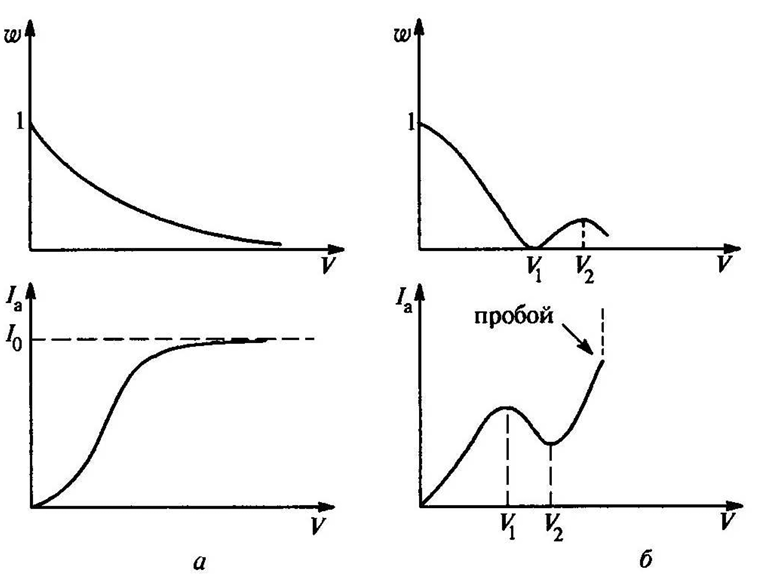
\includegraphics[width=0.6\textwidth]{1.png}
    % \fbox{\parbox{0.8\textwidth}{\centering\vspace{2cm} \textit{Вставьте сюда Рис. 2 из методички: ВАХ тиратрона при классическом (а) и квантовом (б) рассмотрении} \vspace{2cm}}}
    \caption{Вольт-амперная характеристика тиратрона: (а) классическое рассмотрение, (б) квантовое рассмотрение с эффектом Рамзауэра.}
    \label{fig:vax}
\end{figure}

Согласно формуле (5), по измеренной ВАХ тиратрона можно определить зависимость вероятности рассеяния электрона от его энергии из соотношения:
\begin{equation}
    w(V) = -\frac{1}{C} \ln\frac{I_a(V)}{I_0}.
\end{equation}

\subsection*{4. Методы измерения}
В работе используются два режима измерения ВАХ:

\textbf{Динамический режим:} На лампу подаётся синусоидальное напряжение частоты 50 Гц. Сигнал подаётся на электронный осциллограф, на экране которого наблюдается зависимость $I_a = f(V)$. В этом режиме можно надёжно наблюдать лишь первый минимум в сечении рассеяния и следующий за ним максимум.

\textbf{Статический режим:} Напряжение изменяется медленно и вручную, ток измеряется вольтметром. Этот режим позволяет получить более точные данные, особенно в областях максимума и минимума характеристики.

\subsection*{5. Определение параметров атома}
Из условия первого максимума коэффициента прохождения ($n = 1$) при известной глубине ямы $U_0 = 2,5$ В можно определить размер электронной оболочки атома $l$:
\begin{equation}
    l = \frac{\hbar \pi}{\sqrt{2m(E_1 + U_0)}}.
\end{equation}

Глубину потенциальной ямы можно оценить по положению первого минимума сечения рассеяния (первого максимума ВАХ):
\begin{equation}
    U_0 \approx E_{\text{max}}.
\end{equation}

Потенциал ионизации газа определяется по напряжению пробоя тиратрона, при котором происходит резкий скачок тока.





\section*{Ход работы}

\subsection*{1. ВАХ тиратрона в динамическом режиме}

В динамическом режиме на тиратрон подавалось синусоидальное напряжение частотой 50 Гц. Сигнал напряжения «катод--сетка» подавался на вход X осциллографа, а сигнал, пропорциональный анодному току, --- на вход Y. 

Измерения проводились для двух значений напряжения накала. На экране наблюдались первый максимум, следующий за ним минимум и резкий скачок тока, соответствующий пробою. Также проверено влияние магнитного поля: при поднесении магнита ВАХ искажалась из-за отклонения рассеянных электронов силой Лоренца.

Результаты измерений характерных точек представлены в таблице 1.

\begin{table}[H]
\centering
\caption{Характерные точки ВАХ в динамическом режиме}
\label{tab:dynamic_vax}
\renewcommand{\arraystretch}{1.3}
\begin{tabular}{|c|c|c|c|}
\hline
$U_{\text{нак}}$, В & $U_{\text{макс}}$, В & $U_{\text{мин}}$, В & $U_{\text{пробоя}}$, В \\
\hline
$2,753 \pm 0,002$ & $4,0 \pm 0,8$ & $10,2 \pm 0,8$ & $14,8 \pm 0,8$ \\
$2,918 \pm 0,002$ & $4,8 \pm 0,8$ & $10,0 \pm 0,8$ & $14,8 \pm 0,8$ \\
\hline
\end{tabular}
\end{table}

\begin{figure}[H]
    \centering
    \begin{subfigure}{0.48\textwidth}
        \centering
        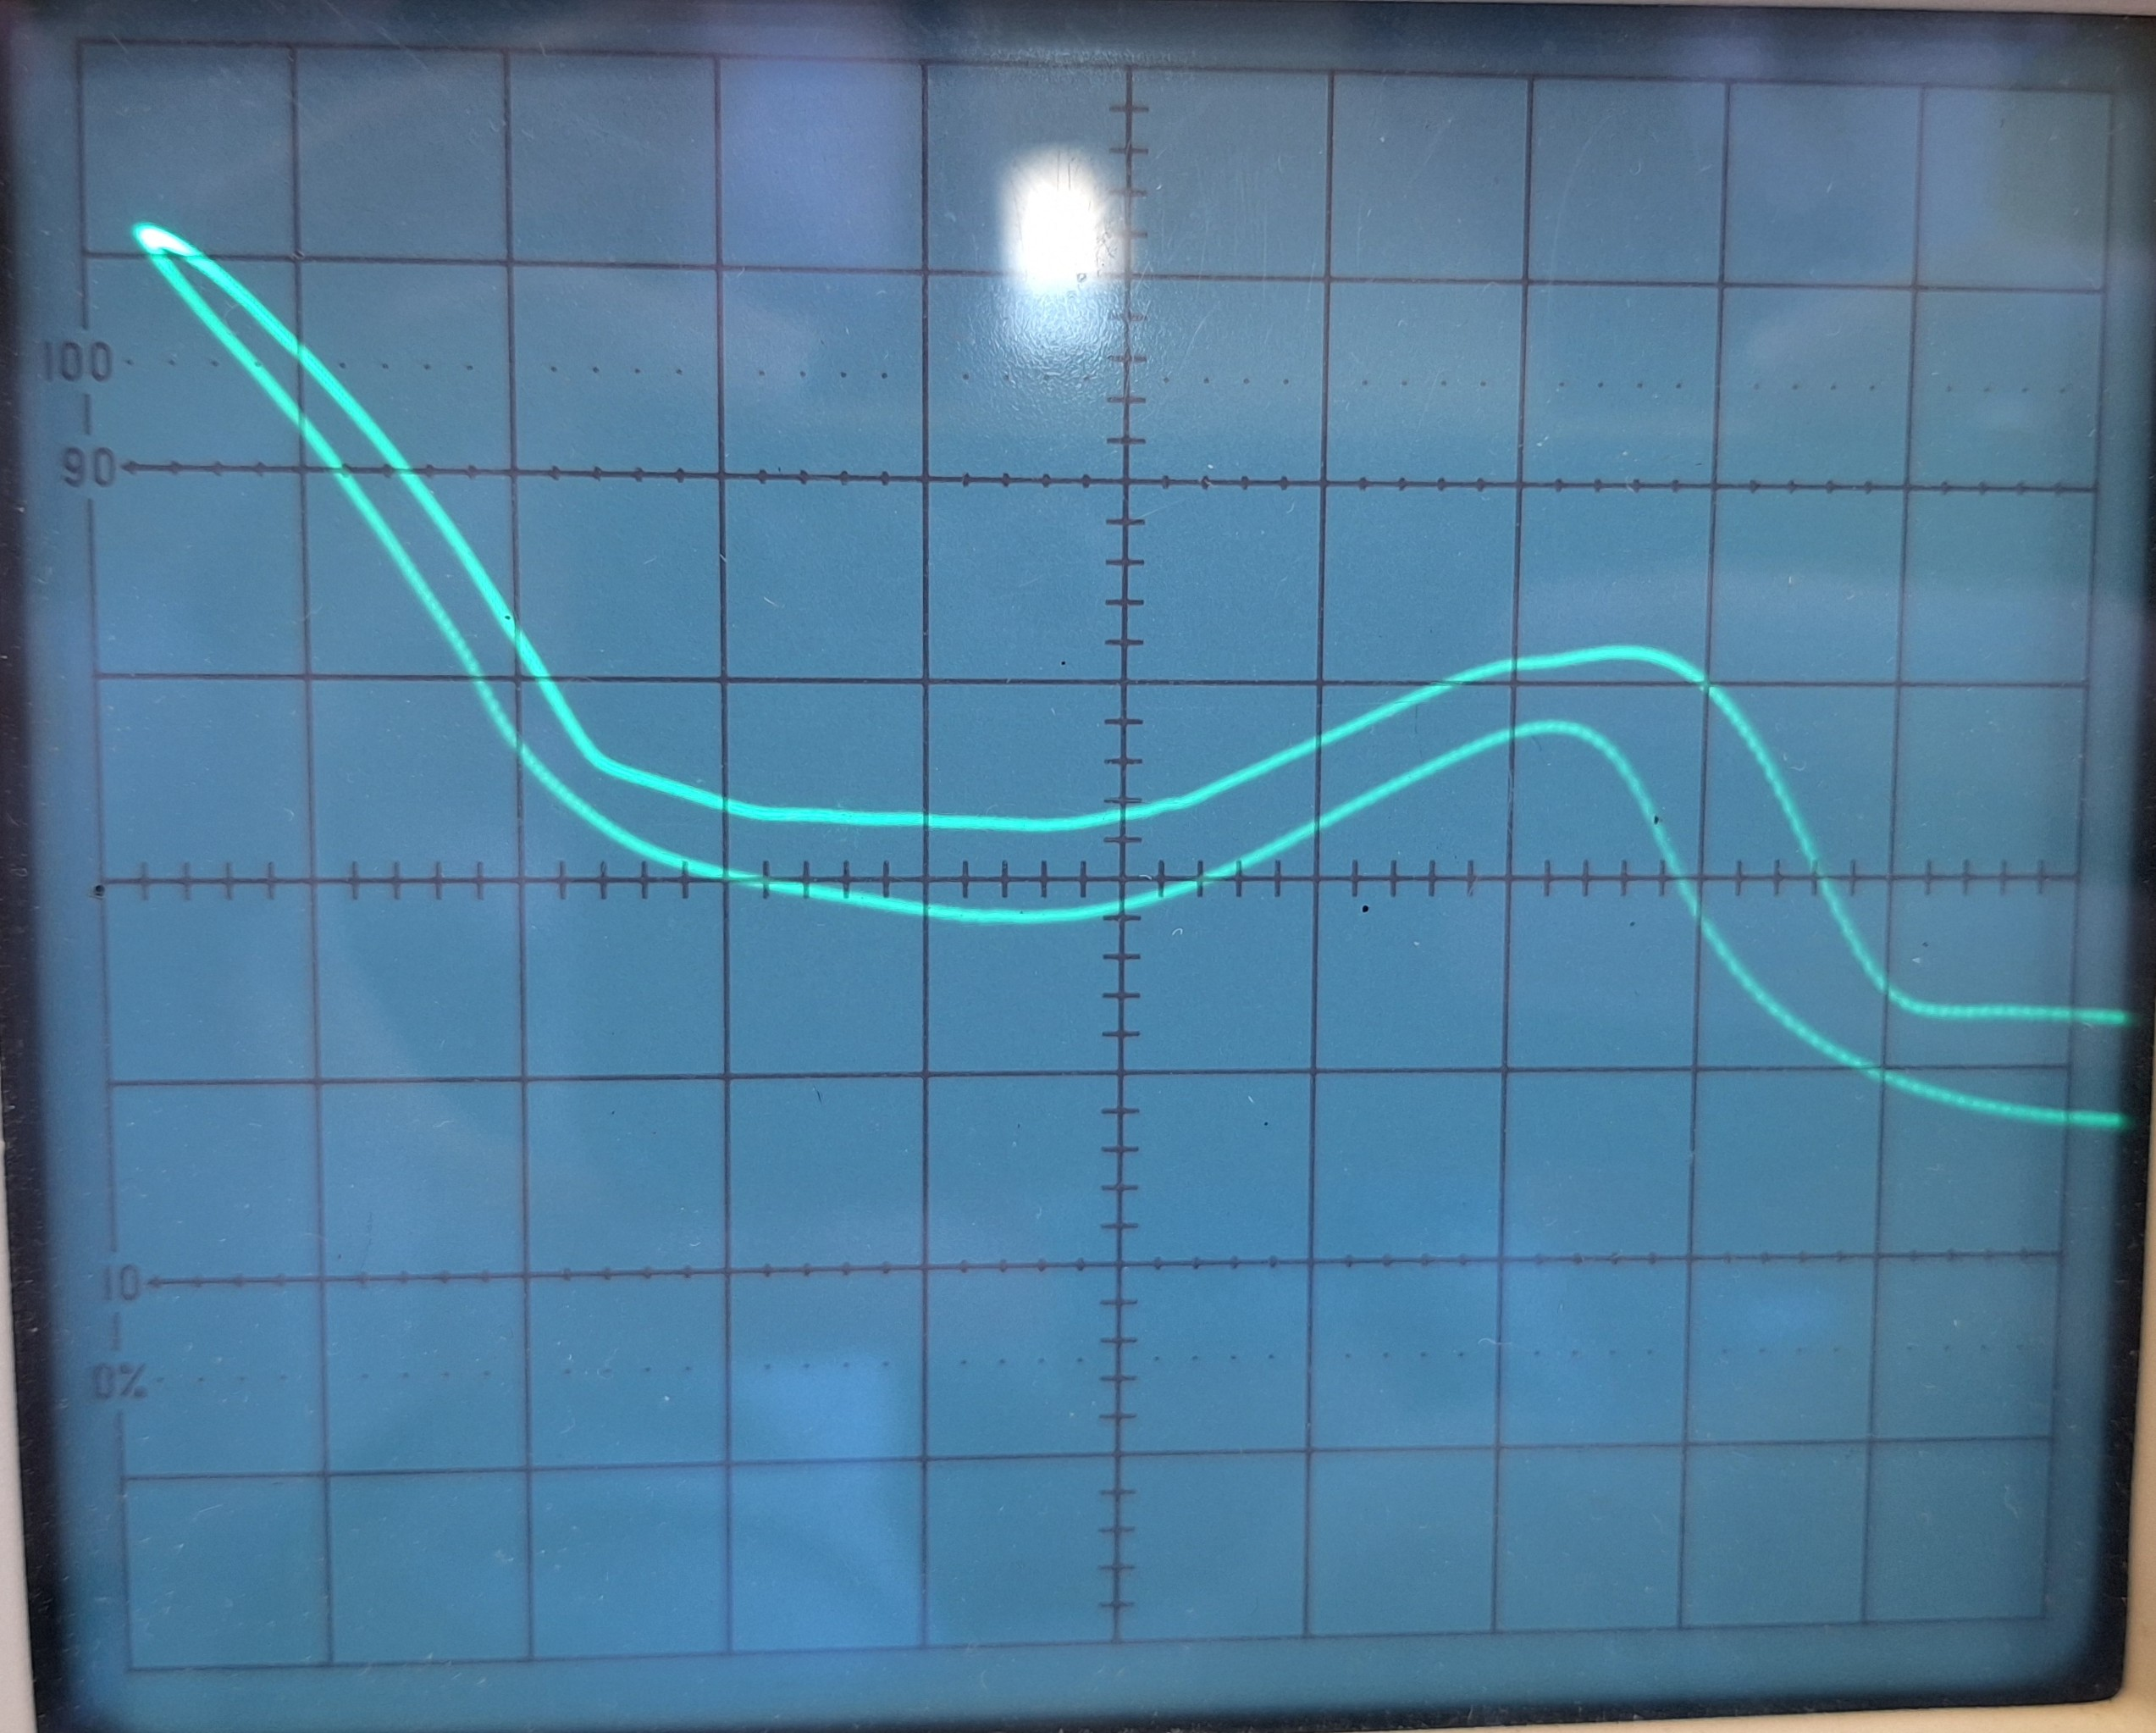
\includegraphics[width=\textwidth]{2.jpg}
        \caption{$U_{\text{нак}} = 2,753$ В}
        \label{fig:osc_2_75}
    \end{subfigure}
    \hfill
    \begin{subfigure}{0.48\textwidth}
        \centering
        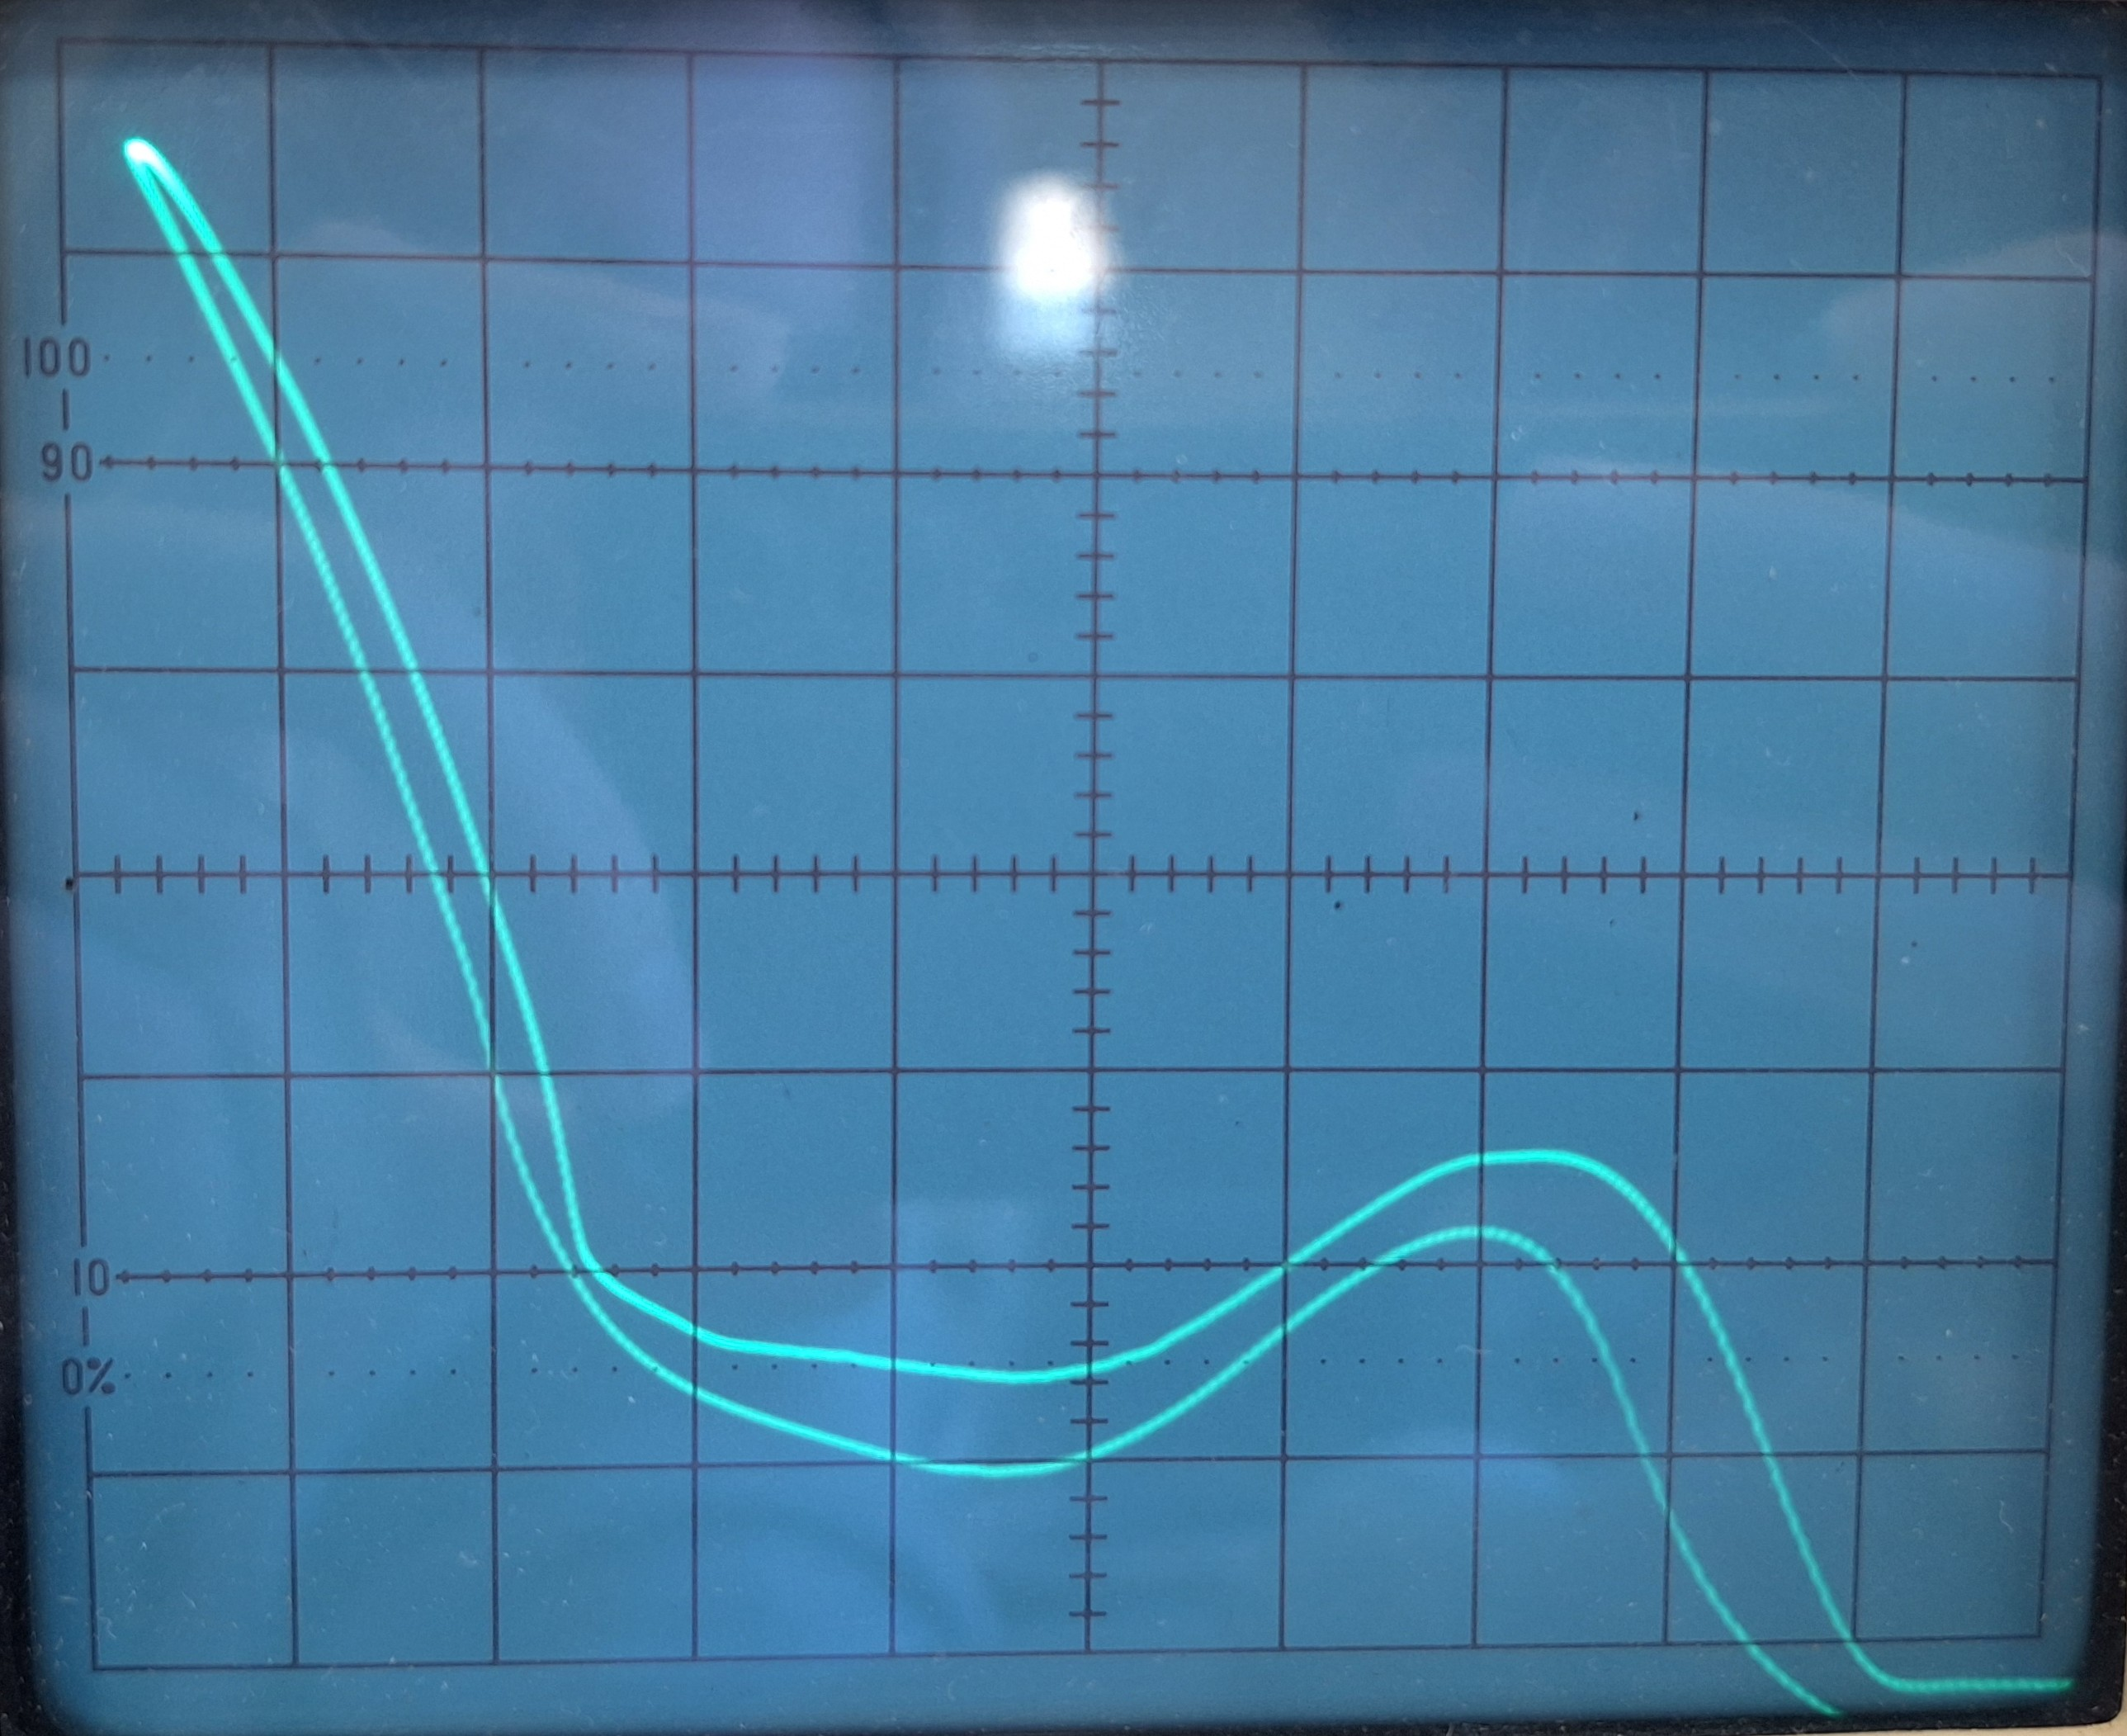
\includegraphics[width=\textwidth]{3.jpg}
        \caption{$U_{\text{нак}} = 2,918$ В}
        \label{fig:osc_2_91}
    \end{subfigure}
    \caption{Осциллограммы ВАХ тиратрона в динамическом режиме.}
    \label{fig:oscilloscope_pair}
\end{figure}

\begin{figure}[H]
    \centering
    \begin{subfigure}{0.3\textwidth}
        \centering
        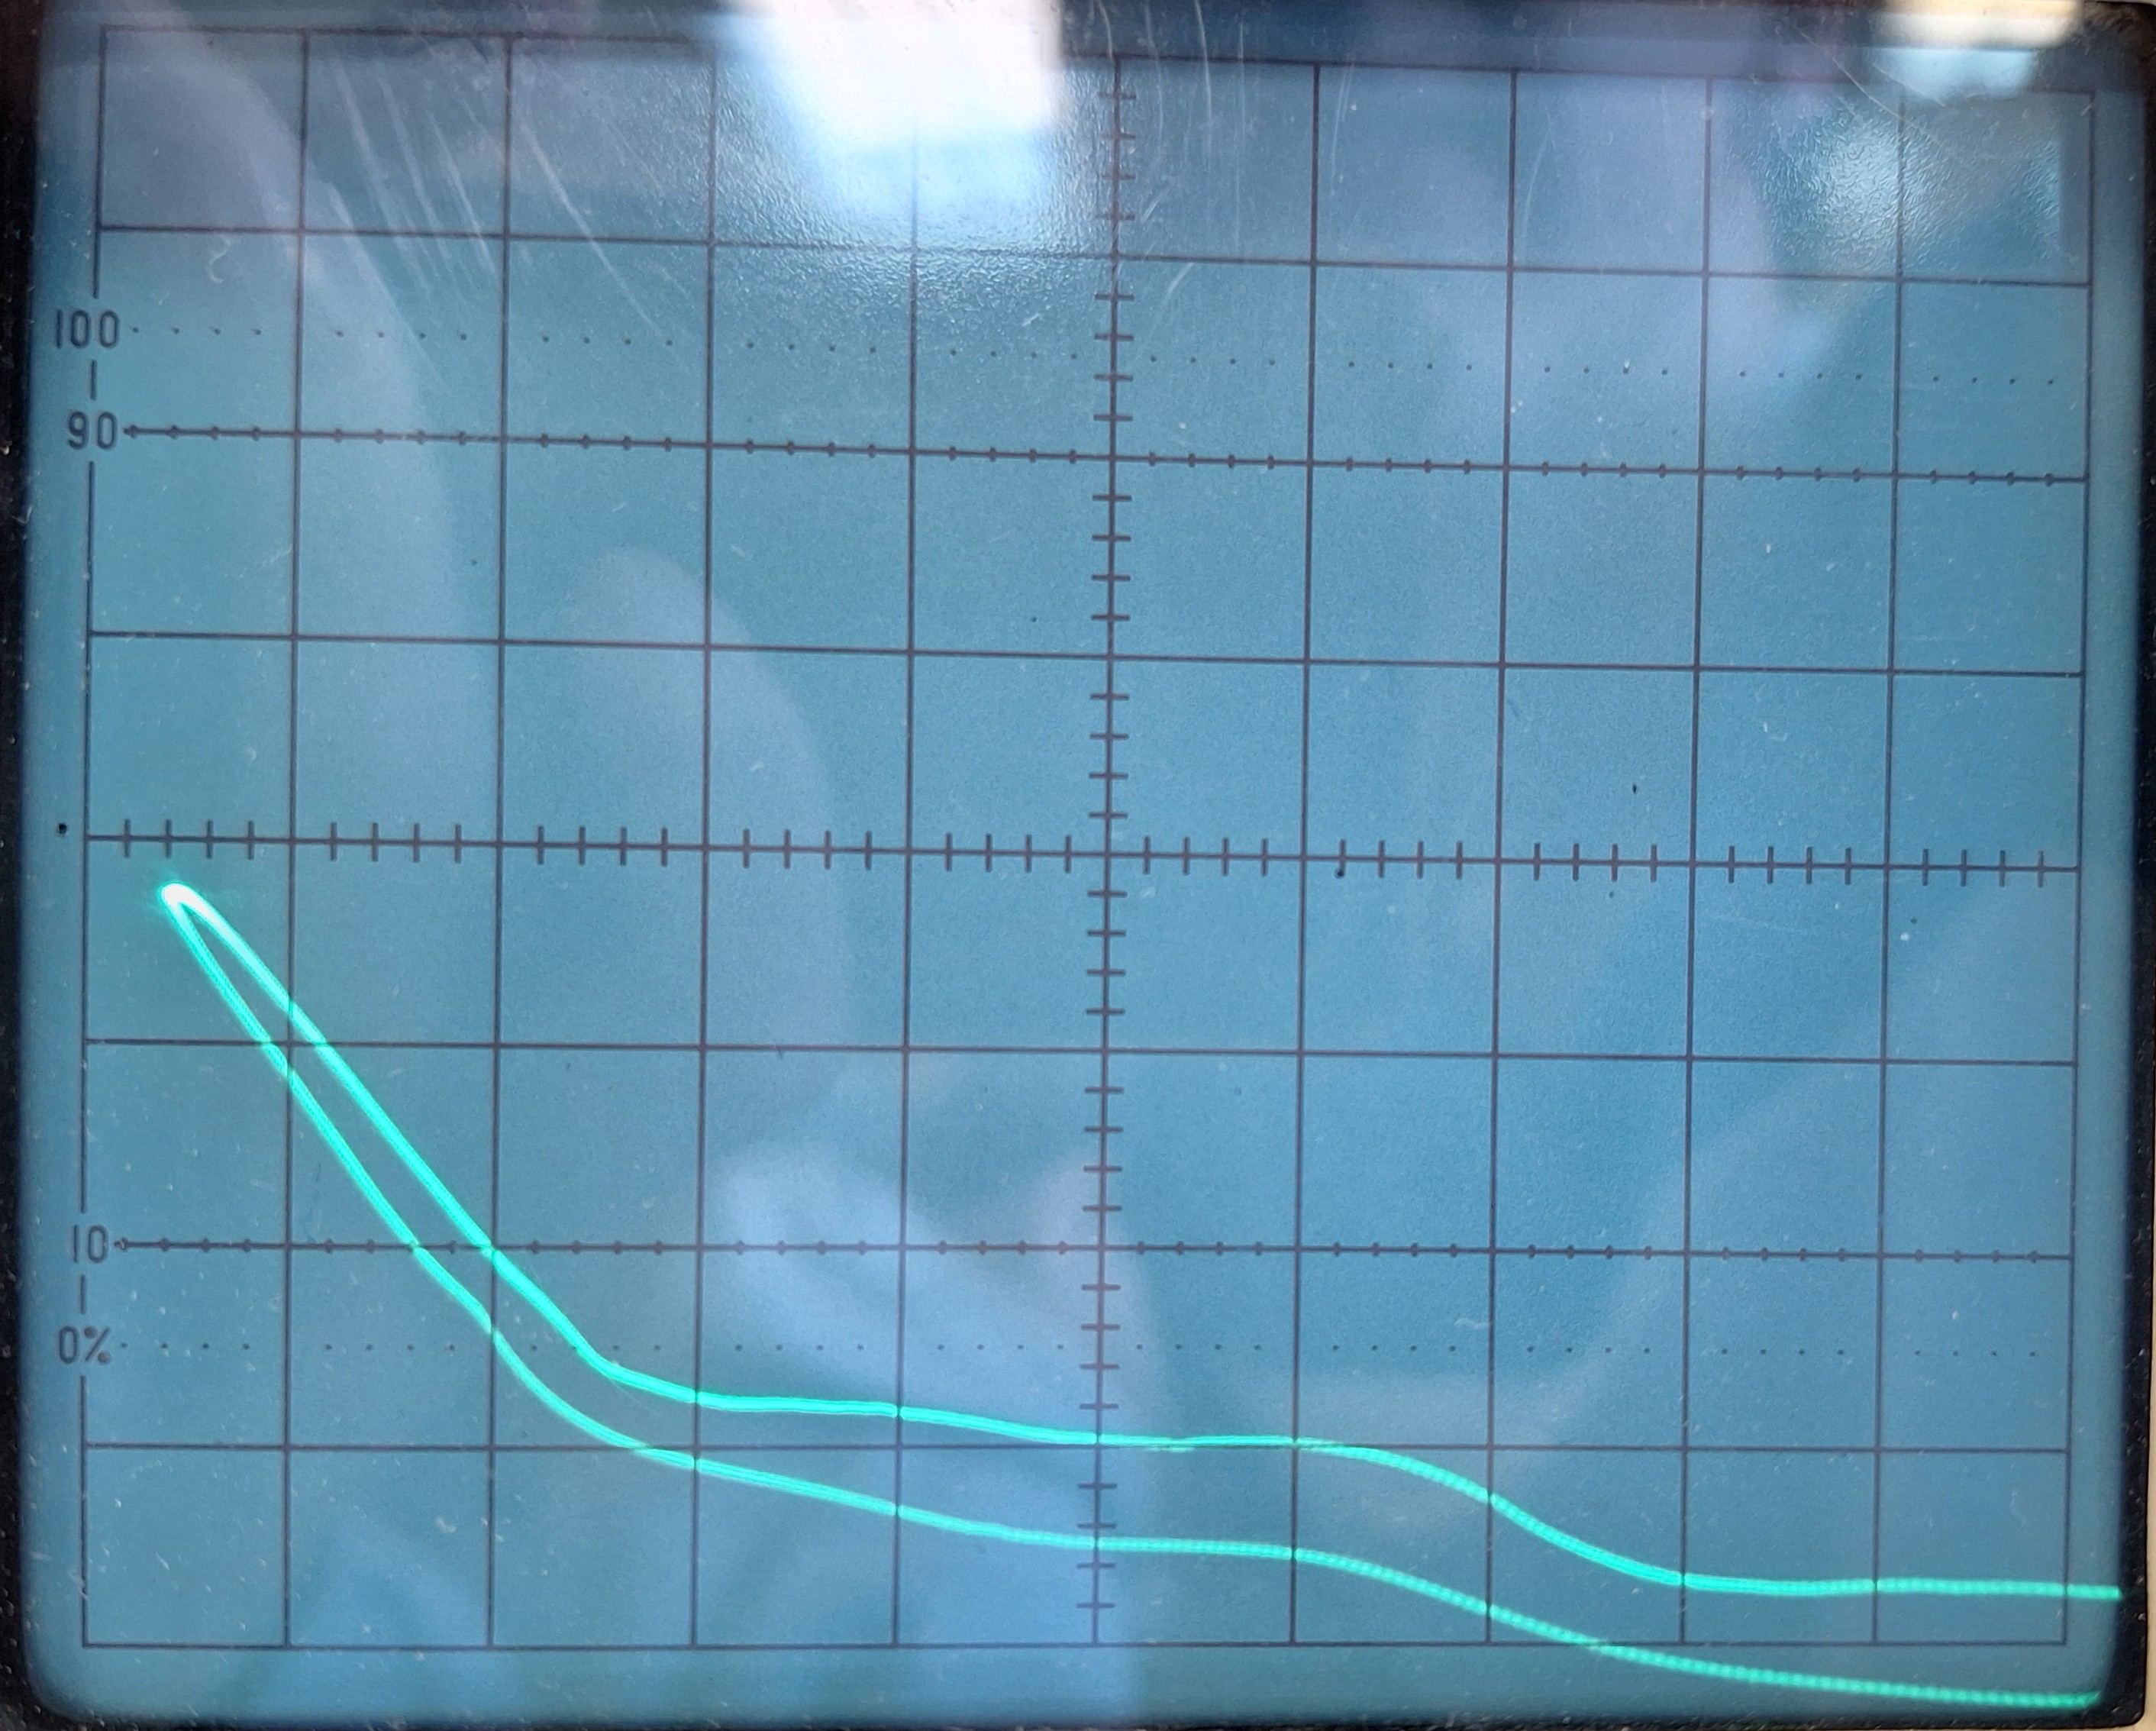
\includegraphics[width=\textwidth]{4 1.jpg}
    \end{subfigure}\hspace{0.02\textwidth}%
    \begin{subfigure}{0.3\textwidth}
        \centering
        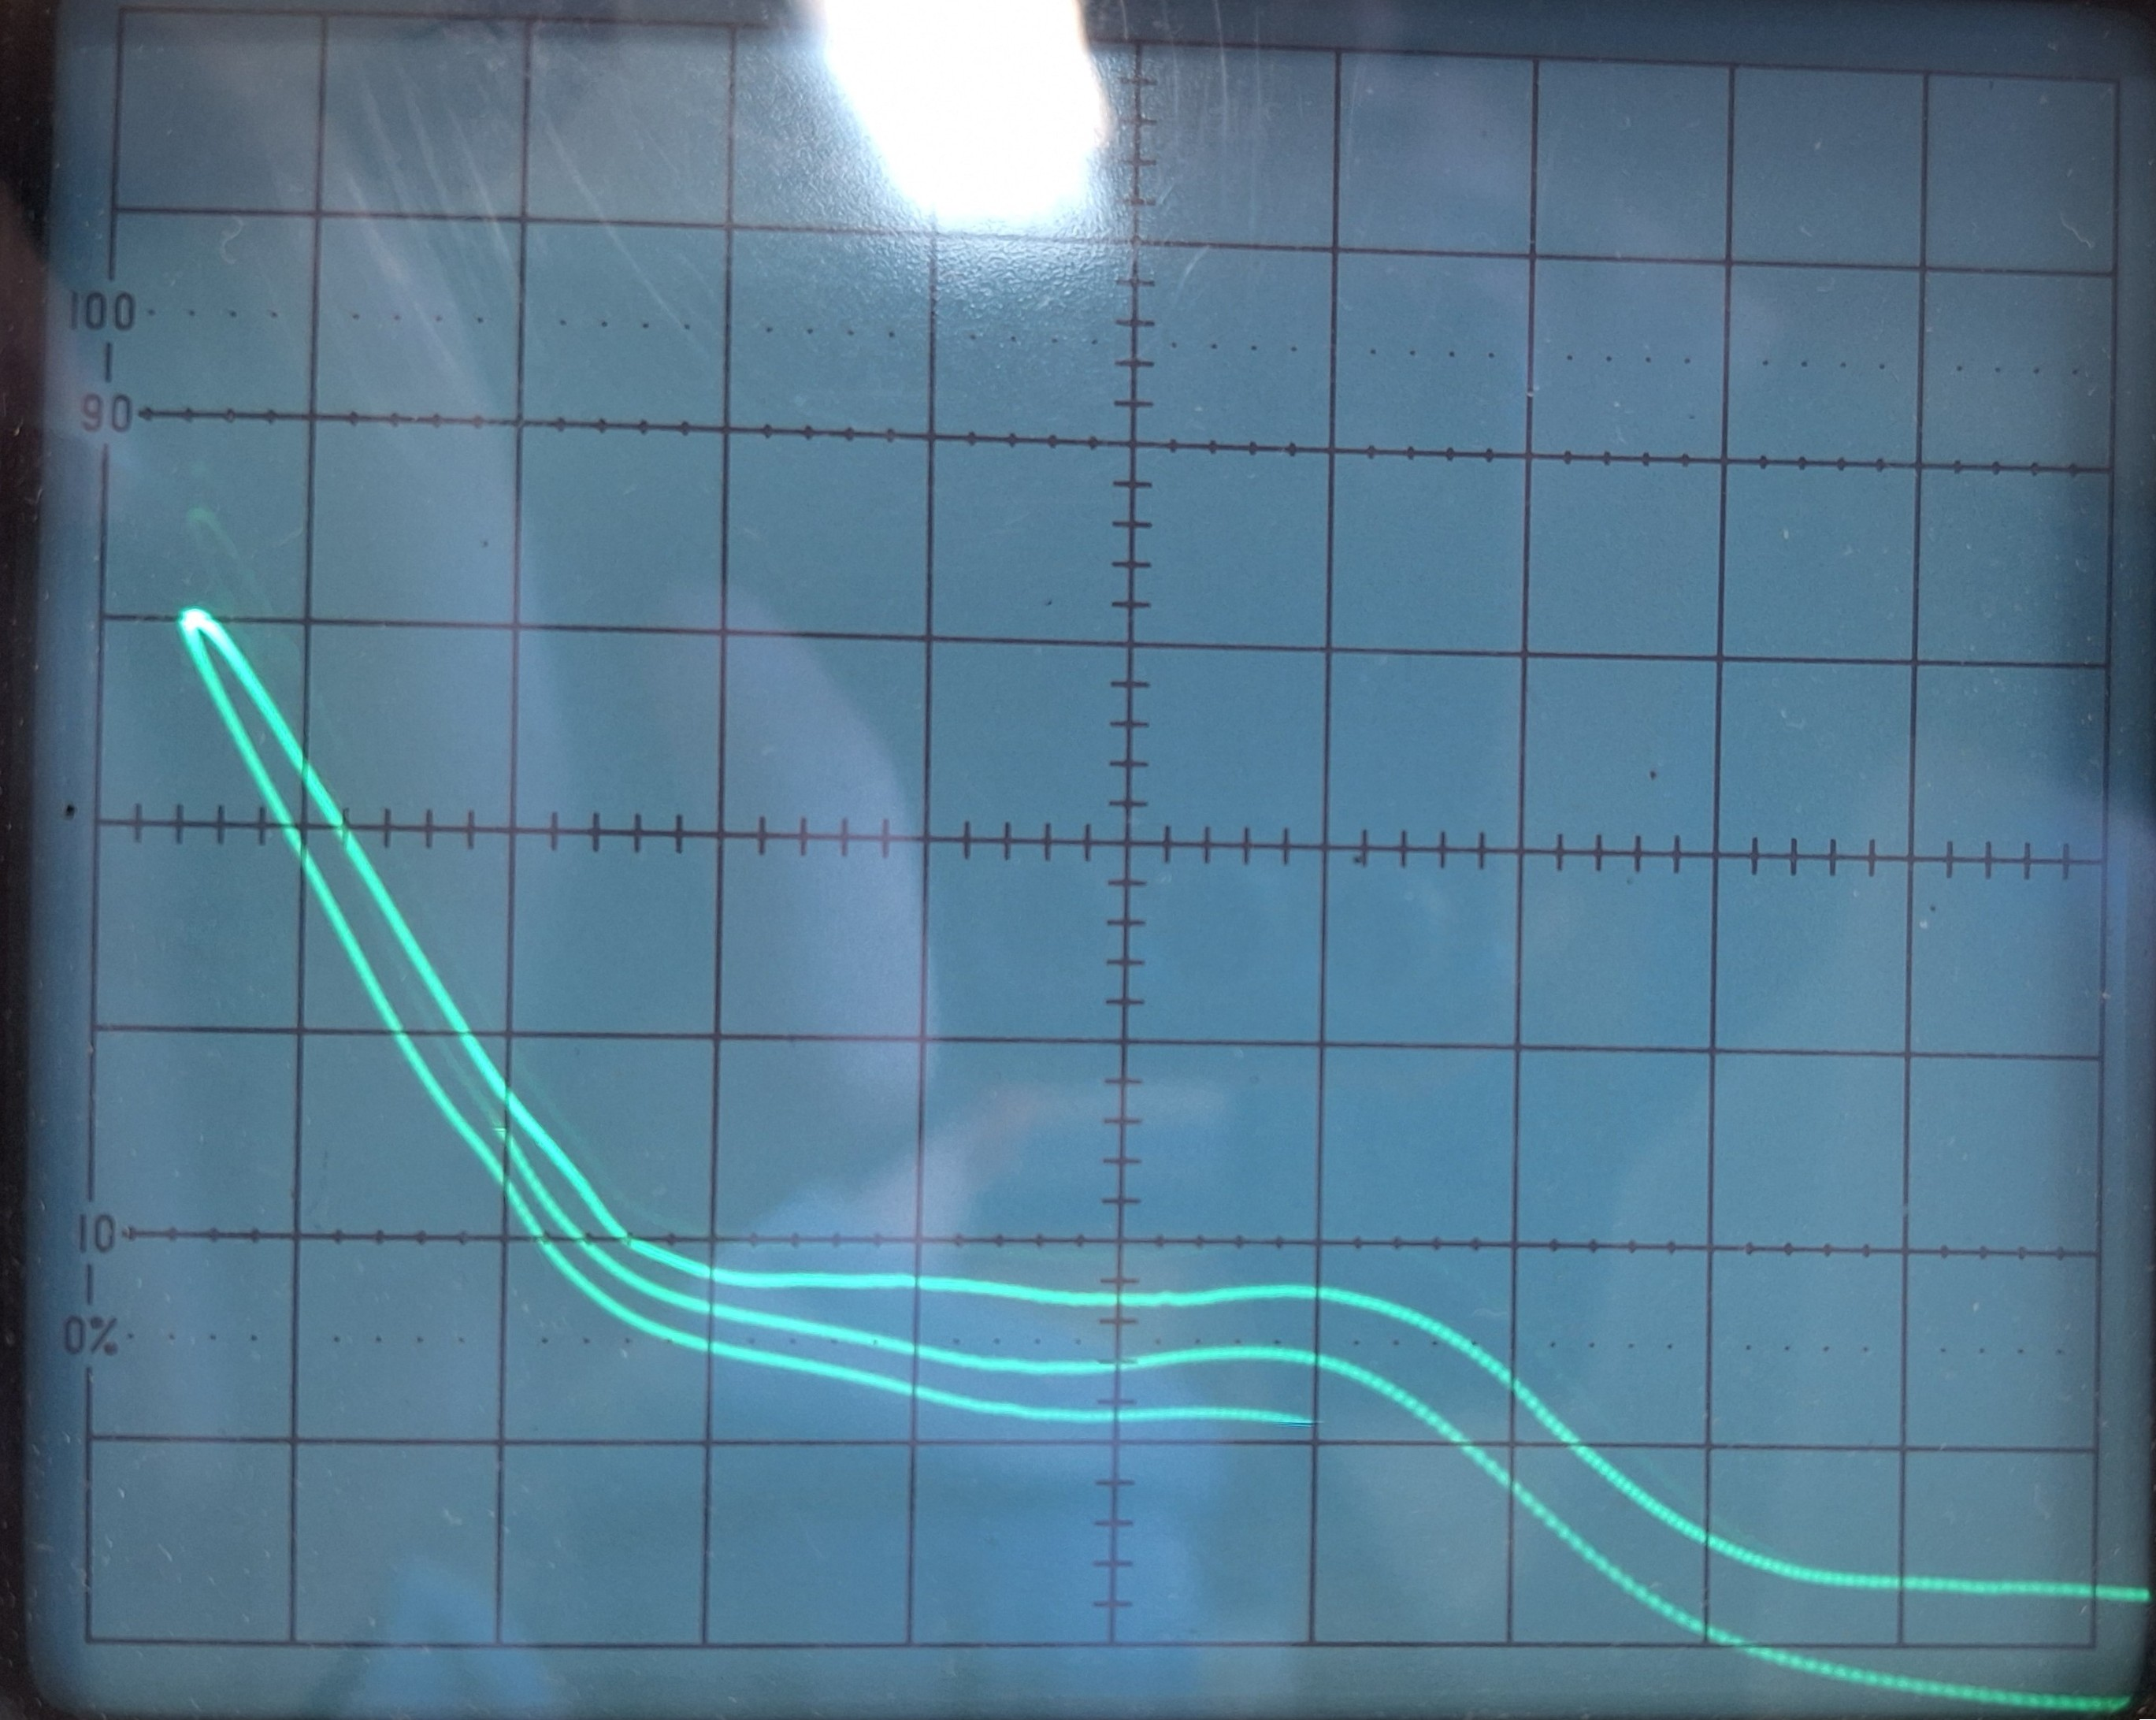
\includegraphics[width=\textwidth]{4 2.jpg}
    \end{subfigure}\hspace{0.02\textwidth}%
    \begin{subfigure}{0.3\textwidth}
        \centering
        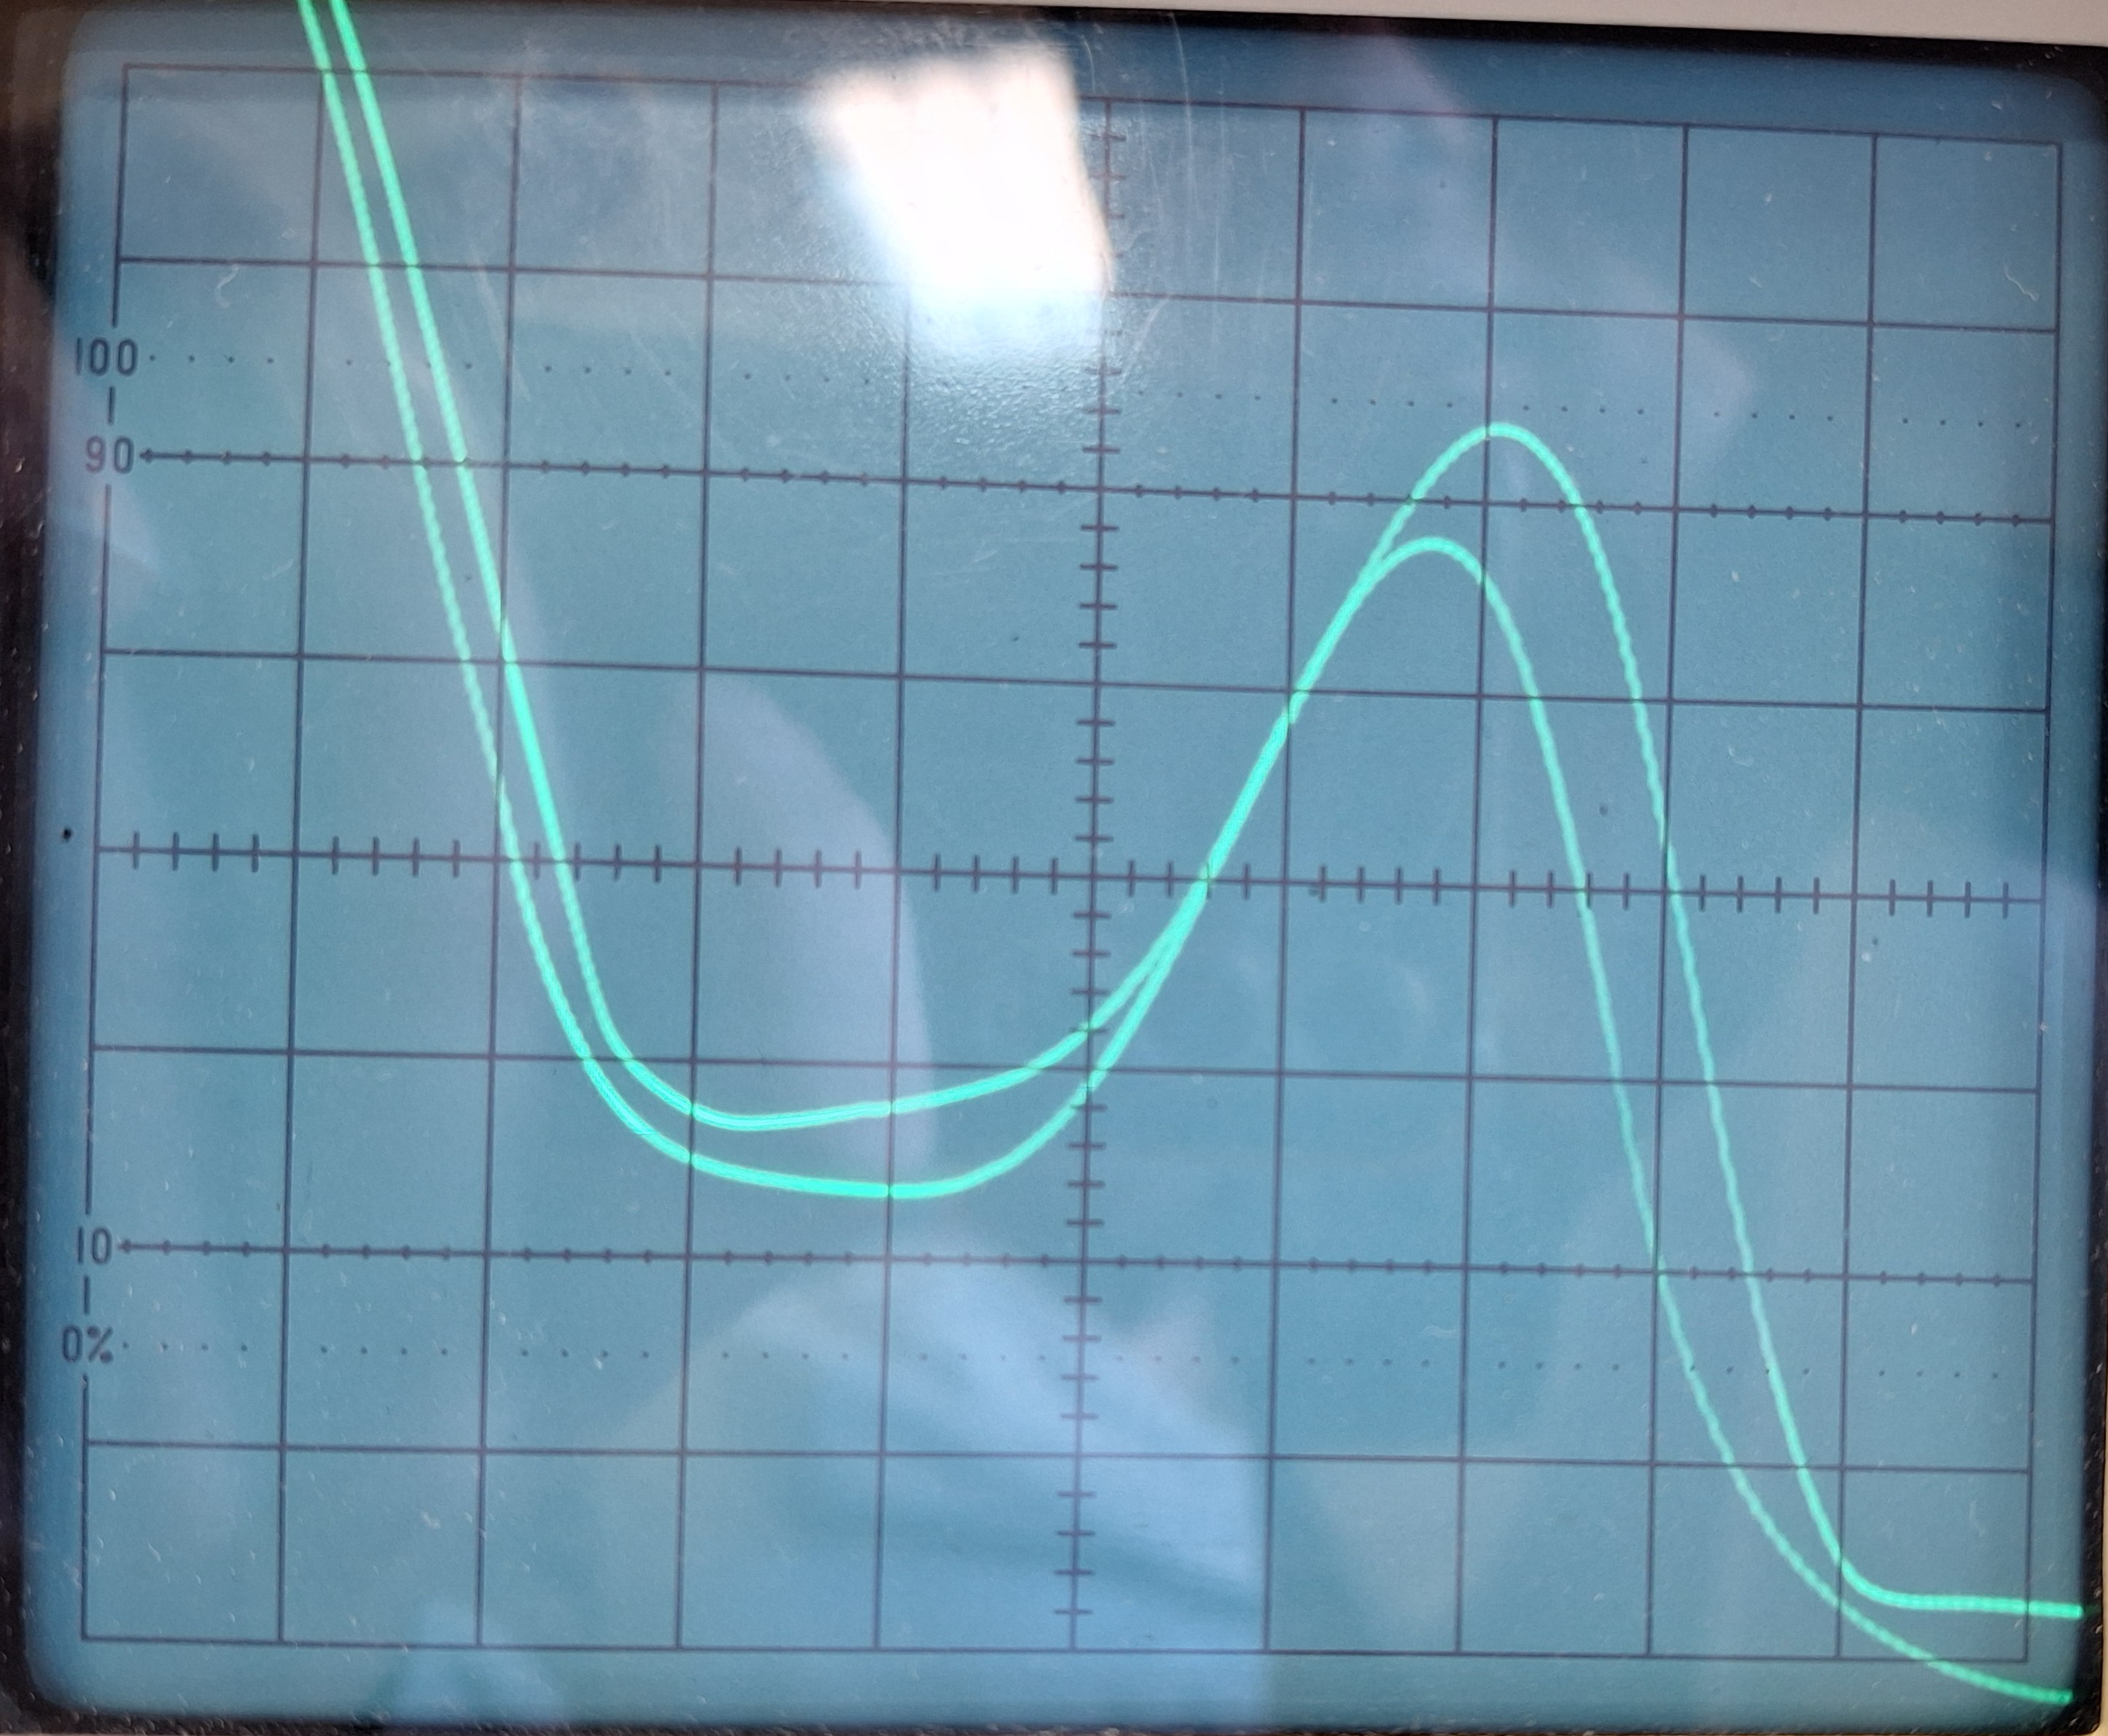
\includegraphics[width=\textwidth]{4 3.jpg}
    \end{subfigure}
    \caption{Изменение ВАХ под действием магнитного поля при различной ориентации магнита.}
    \label{fig:oscilloscope_magnet}
\end{figure}

\subsection*{2. ВАХ тиратрона в статическом режиме}

Измерения проводились при плавном увеличении ускоряющего напряжения $V$. Анодный ток $I_a$ определялся по показаниям вольтметра, включенного параллельно резистору $R = 100$ кОм: $I_a = V_{\text{анод}} / R$. Измерения в областях экстремумов проводились с меньшим шагом.

\begin{table}[H]
\centering
\caption{Фрагмент данных ВАХ в статическом режиме}
\label{tab:static_vax}
\renewcommand{\arraystretch}{1.2}
\begin{tabular}{|c|c|c|c|}
\hline
\multicolumn{2}{|c|}{$U_{\text{нак}} = 2,755$ В} & \multicolumn{2}{c|}{$U_{\text{нак}} = 2,925$ В} \\
\hline
$V$, В & $I_a$, мкА & $V$, В & $I_a$, мкА \\
\hline
3,712 & 0,47 & 5,031 & 0,67 \\
5,328 & 0,44 & 5,543 & 0,67 \\
9,837 & 0,21 & 10,188 & 0,39 \\
11,979 & 0,23 & 11,523 & 0,42 \\
\hline
\end{tabular}
\end{table}

\begin{figure}[H]
    \centering
    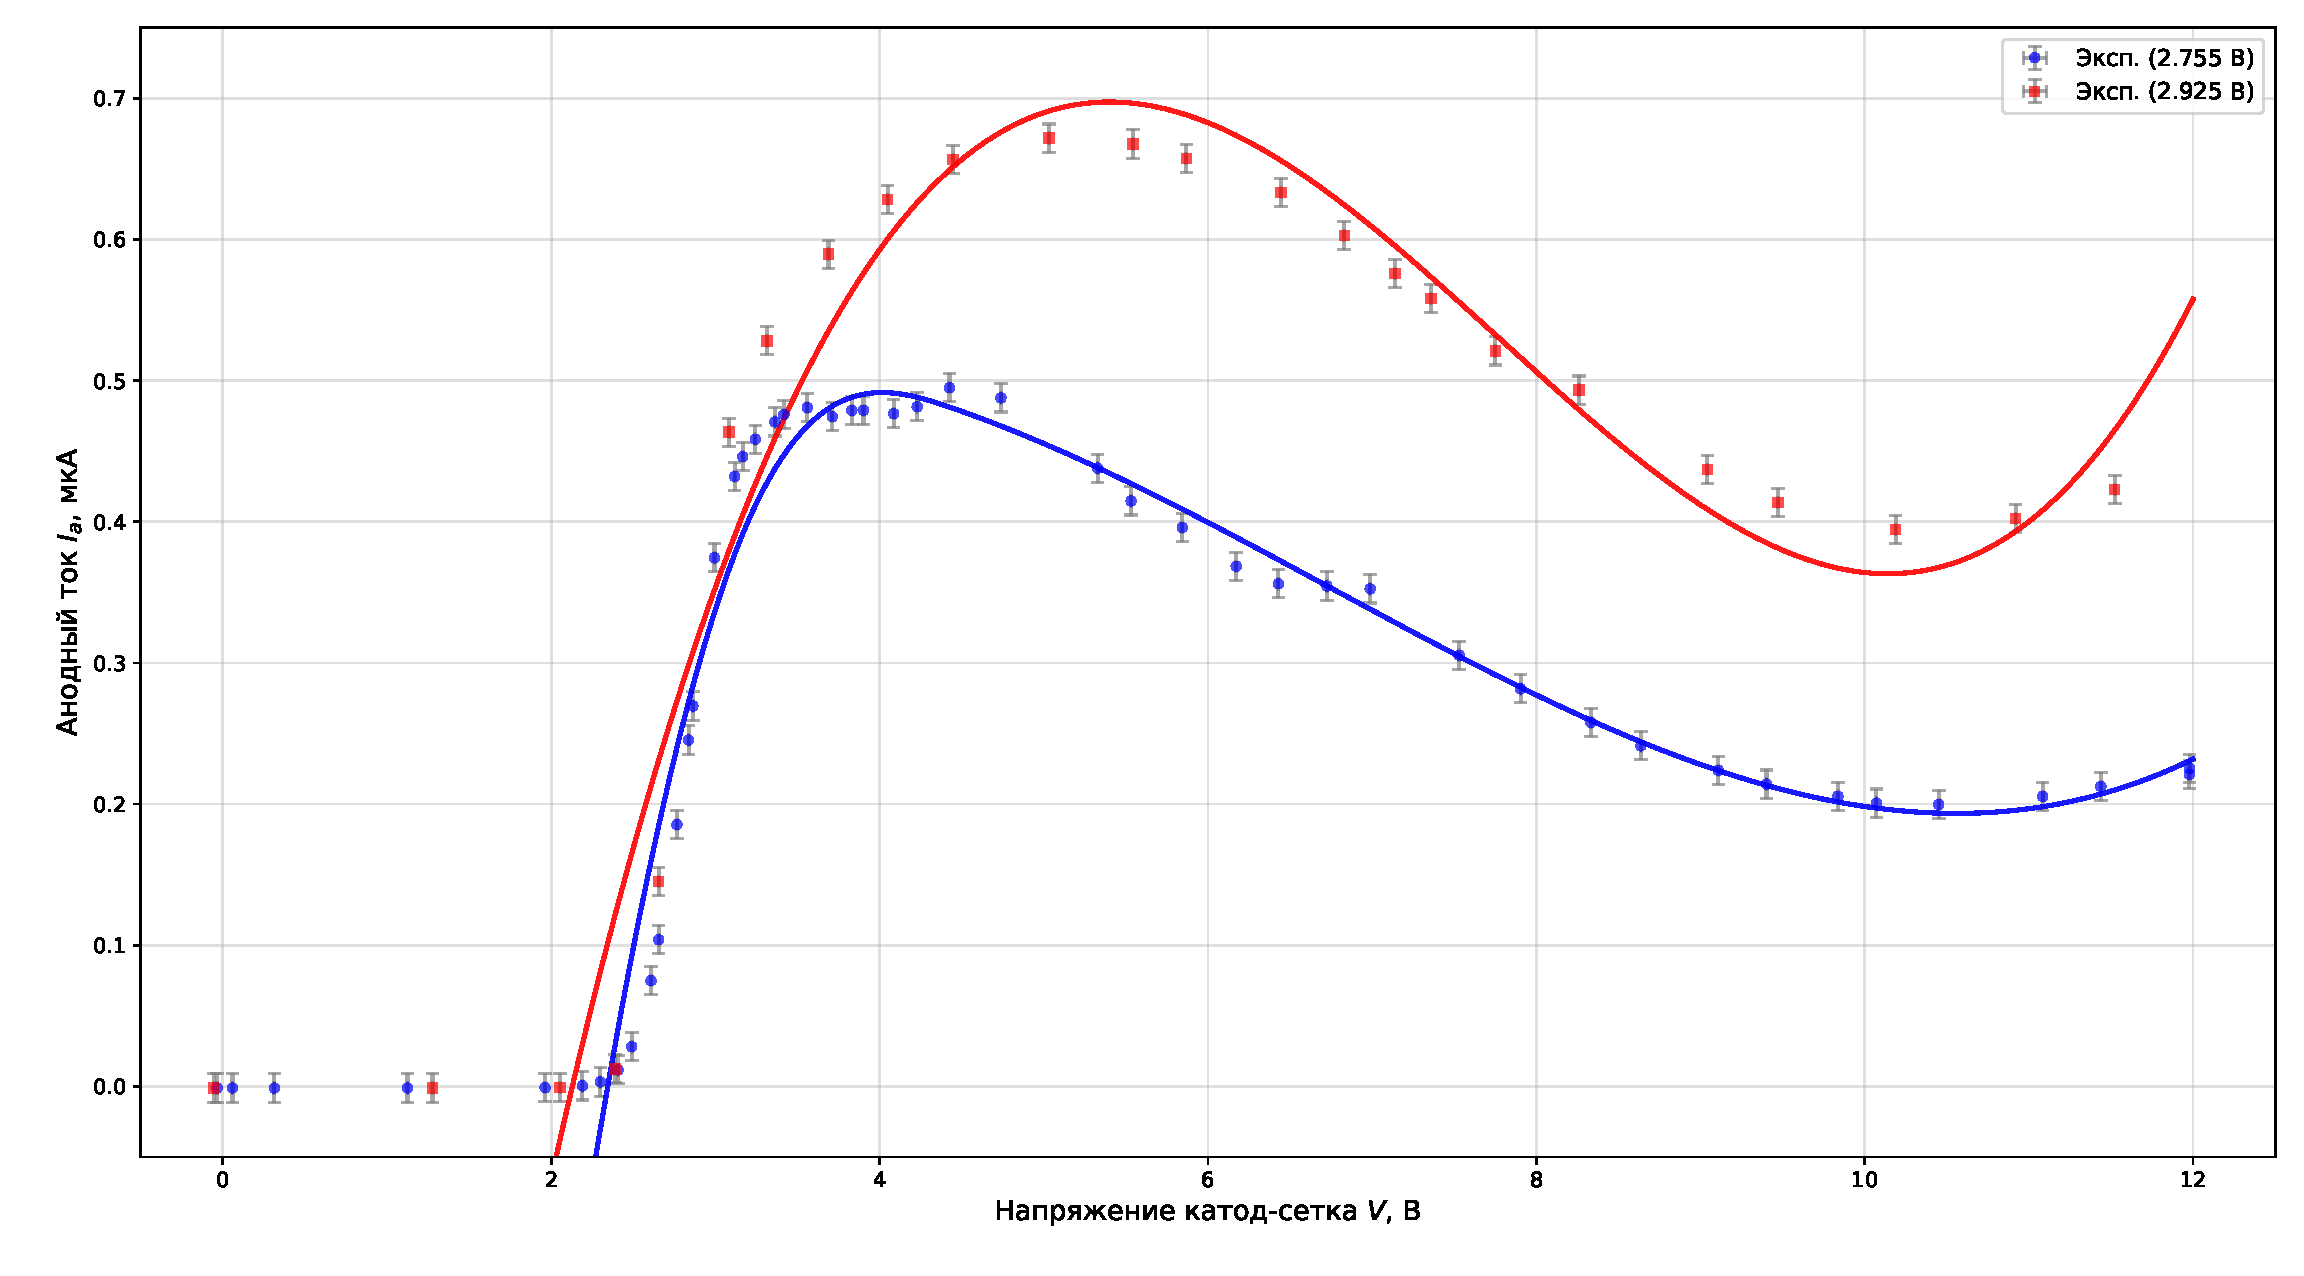
\includegraphics[width=0.8\textwidth]{5.pdf}
    \caption{ВАХ тиратрона в статическом режиме для двух значений напряжения накала.}
    \label{fig:vax_static}
\end{figure}

\subsection*{3. Обработка результатов}

\subsubsection*{3.1. Определение размера электронной оболочки атома}
Из графика на рис. \ref{fig:vax_static} определены положения первого максимума ВАХ: $V_{\text{макс}} \approx 3,7$ В (для $2,755$ В) и $5,0$ В (для $2,925$ В). Среднее значение $V_{\text{макс.ср}} = 4,35 \pm 0,14$ В.

Используя формулу для резонансного прохождения через яму глубиной $U_0 = 2,5$ эВ:
\begin{equation}
    l = \frac{h}{2\sqrt{2m_e e (V_{\text{макс.ср}} + U_0)}},
\end{equation}
получаем размер оболочки: $l \approx 2,34 \cdot 10^{-10}$ м $= 2,34$ \AA. 
Погрешность $\frac{\Delta l}{l} = \frac{1}{2} \frac{\Delta V_{\text{макс.ср}}}{V_{\text{макс.ср}} + U_0} \approx 0,01$, откуда $\Delta l \approx 0,03$ \AA. 
Итог: $l = (2,34 \pm 0,03)$ \AA.

Согласно заданию, рассчитаем $l$ по упрощённой формуле, исключая $U_0$ (полагая $E \gg U_0$):
\begin{equation}
    l' = \frac{h}{2\sqrt{2m_e e V_{\text{макс.ср}}}} \approx 2,94 \text{ \AA}.
\end{equation}
Оба значения ($2,34$ \AA\ и $2,94$ \AA) имеют правильный порядок величины и согласуются с табличными радиусами инертных газов (Ar: $1,88$ \AA, Kr: $2,02$ \AA, Xe: $2,16$ \AA), что подтверждает модель потенциальной ямы.

\subsubsection*{3.2. Оценка глубины потенциальной ямы}
Согласно формуле (9), глубина ямы оценивается как $U_0 \approx E_{\text{макс}} = e V_{\text{макс.ср}}$. 
Для динамического режима $V_{\text{макс.ср}} = 4,4 \pm 0,6$ В, для статического --- $4,35 \pm 0,6$ В. 
Средняя оценка: $U_0 \approx 4,4 \pm 0,6$ эВ. Это значение превышает $2,5$ эВ, использованное в п. 3.1, что объясняется приближённым характером формулы (9), не учитывающей точную форму потенциала.

\subsubsection*{3.3. Определение потенциала ионизации}
Напряжение пробоя в динамическом режиме составило $14,8 \pm 0,8$ В, а в статическом (по началу роста тока после минимума) --- $11,5 \pm 0,5$ В. 
С учётом контактной разности потенциалов ($\sim 0,5$--$1,0$ В), истинный потенциал ионизации лежит в диапазоне $12,0$--$15,8$ эВ. Сопоставляя с табличными данными (Ar: $15,8$ эВ, Kr: $14,0$ эВ, Xe: $12,1$ эВ), можно сделать вывод, что тиратрон заполнен криптоном или ксеноном (либо их смесью).

\subsubsection*{3.4. Оценка положений максимумов для $n = 2, 3$}
Из условия $k_2 l = n\pi$ следует зависимость энергии $n$-го максимума от первого:
\begin{equation}
    E_n = n^2 E_1 + (n^2 - 1)U_0.
\end{equation}
Подставляя $E_1 = 4,35$ В и $U_0 = 2,5$ эВ, получаем:
\begin{equation}
    E_2 = 4 \cdot 4,35 + 3 \cdot 2,5 = 24,9 \text{ В}, \quad E_3 = 9 \cdot 4,35 + 8 \cdot 2,5 = 59,15 \text{ В}.
\end{equation}
На экспериментальных ВАХ эти максимумы не наблюдаются. Это согласуется с методичкой: при таких напряжениях происходит ионизация газа и пробой тиратрона, а глубина минимума сечения рассеяния с ростом $n$ резко уменьшается.

\subsubsection*{3.5. Зависимость вероятности рассеяния от энергии}
Согласно формуле (12), вероятность рассеяния связана с ВАХ как $w(V) = -\frac{1}{C} \ln \frac{I_a(V)}{I_0}$. 
В качестве $I_0$ (ток без рассеяния) взято максимальное значение анодного тока: $0,495$ мкА (для $2,755$ В) и $0,672$ мкА (для $2,925$ В). 

\begin{figure}[H]
    \centering
    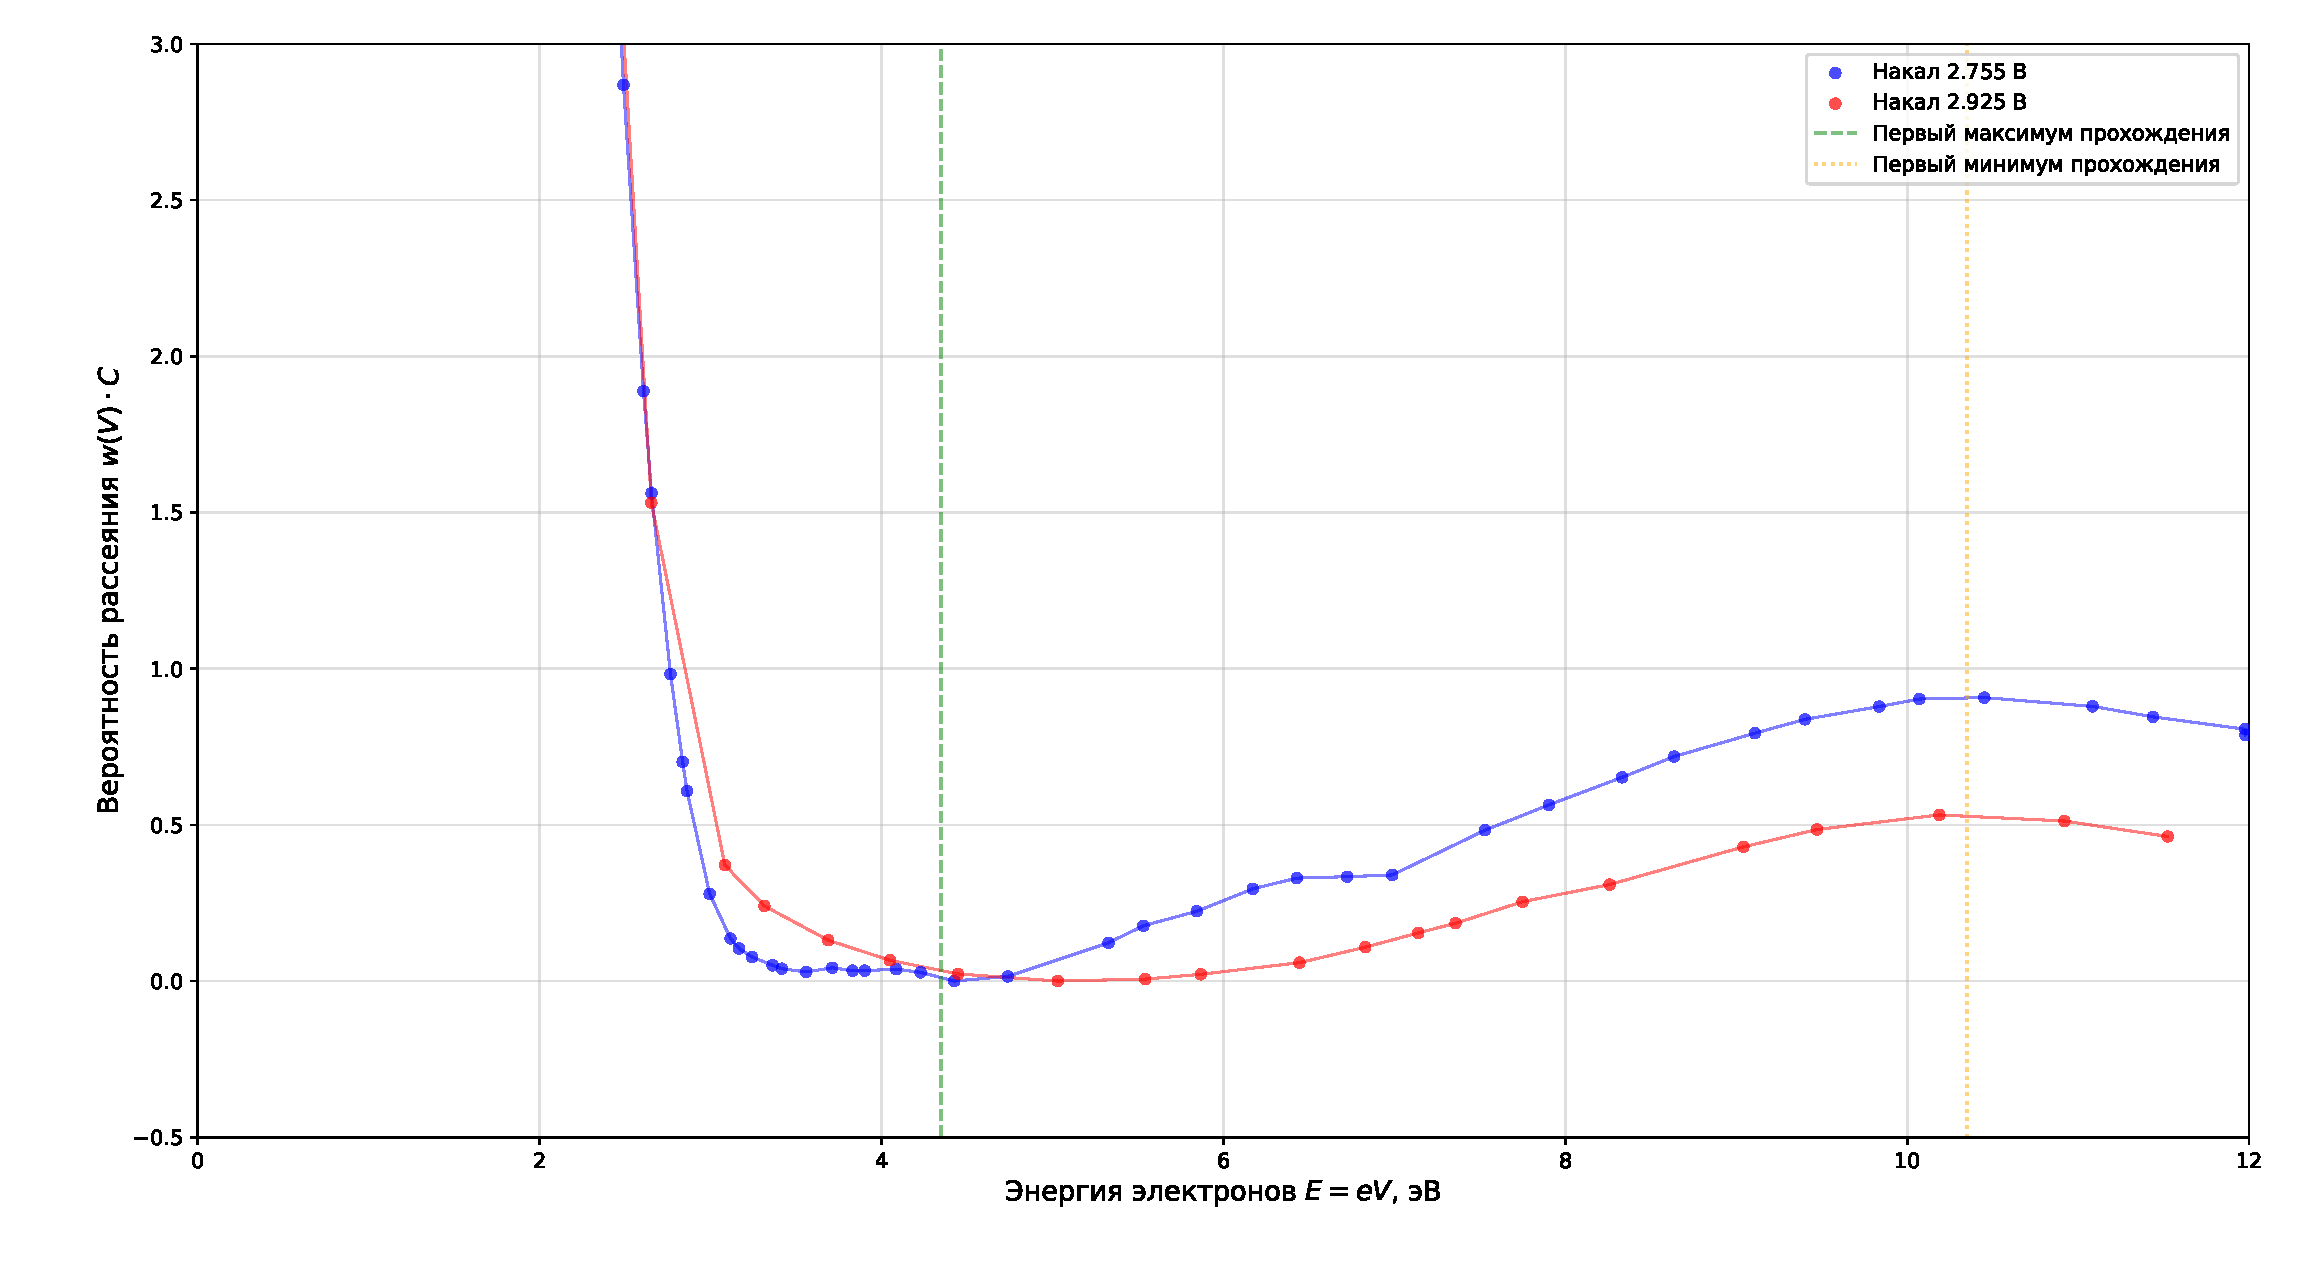
\includegraphics[width=0.8\textwidth]{6.pdf}
    \caption{Зависимость $w(V) \cdot C$ от энергии электронов. Пунктир --- первый максимум прохождения ($V \approx 4,35$ В), штрихпунктир --- минимум ($V \approx 10,35$ В).}
    \label{fig:scattering_probability}
\end{figure}

На рис. \ref{fig:scattering_probability} виден ярко выраженный минимум вероятности рассеяния при $E \approx 4,35$ эВ, что соответствует эффекту Рамзауэра. При дальнейшем росте энергии вероятность рассеяния возрастает, достигая локального максимума при $E \approx 10,35$ эВ. Полученная зависимость качественно согласуется с теоретической кривой.






\section*{Вывод}

В ходе работы была исследована вольт-амперная характеристика тиратрона ТЗ-01/1.3Б в динамическом и статическом режимах. Наблюдается характерный минимум сечения рассеяния при низких энергиях электронов, что подтверждает эффект Рамзауэра и квантовую природу рассеяния.

По положению первого максимума ВАХ ($V_{\text{макс.ср}} = 4,35 \pm 0,14$ В) рассчитан размер электронной оболочки атома:
\begin{equation}
    l = (2,34 \pm 0,03) \text{ \AA} \quad (U_0 = 2,5 \text{ эВ}), \quad l' \approx 2,94 \text{ \AA} \quad (U_0 \text{ исключено}).
\end{equation}
Оба значения имеют правильный порядок величины и согласуются с табличными радиусами инертных газов (Ar: 1,88 \AA, Kr: 2,02 \AA, Xe: 2,16 \AA).

Глубина потенциальной ямы, оценённая по формуле (9), составляет $U_0 \approx 4,4 \pm 0,6$ эВ, что превышает значение 2,5 эВ, использованное при расчёте $l$. Это расхождение объясняется приближённым характером формулы (9).

Напряжение пробоя в динамическом режиме ($14,8 \pm 0,8$ В) и статическом ($11,5 \pm 0,5$ В) позволяет оценить потенциал ионизации газа. С учётом контактной разности потенциалов истинное значение лежит в диапазоне 12--15,8 эВ, что соответствует криптону (14,0 эВ) или ксенону (12,1 эВ).

Максимумы коэффициента прохождения для $n = 2$ ($E_2 \approx 24,9$ В) и $n = 3$ ($E_3 \approx 59,2$ В) на экспериментальных ВАХ не наблюдаются, что согласуется с теорией: при таких напряжениях происходит ионизация газа и пробой тиратрона.

Построенная зависимость вероятности рассеяния от энергии качественно согласуется с теоретической кривой, демонстрируя минимум при $E \approx 4,35$ эВ и максимум при $E \approx 10,35$ эВ.






\end{document}